\documentclass[twoside]{article}
\usepackage[utf8]{inputenc}

% The package supports other formats as well, but this template
% is primarily checked and updated for examinations at TUM BGDM
%\usepackage[uebung, answers]{tumbgdm}

\usepackage[uebung]{tumbgdm}
\usepackage{pythonhighlight}

\Professor{Prof. Dr. Martin Werner}
\Universitaet{Technical University of Munich}
\Institut{School of Engineering and Design}
\Lehrstuhl{Professorship Big Geospatial Data Management}
\Semester[WiTe 2024/25]{Winter Term 2024/25}
\Vorlesung{Principles of Programming}
\InstitutsWebsite{https://www.bgd.lrg.tum.de/}
\VorlesungsWebsite{https://www.moodle.tum.de/course/view.php?id=103704}

\nummerUebungsblatt{5}
\nummerErsteFrage{1}

\LearningOutcome{ Repetition, Turtle graphics, recursion}

\begin{document}
\maketitle

% https://cs111.wellesley.edu/~cs111/archive/cs111_spring15/public_html/notes/lectures/10_turtle_recursion_4up.pdf
% https://codewithsara.com/python-with-sara/python-101/u2-python-turtle-graphics/u2s2-turtle-programming/
% http://opensask.ca/Python/MoreTurtles/DrawingPractice.html
% https://runestone.academy/ns/books/published/fopp/PythonTurtle/Exercises.html

\vspace{10pt}

Python has a built-in module named \code{turtle}, similar to "Niki the robot".
Turtle graphics provide a visualization of a "turtle" with a pen that draws on a sheet of paper on the floor.
It was designed as an educational tool and is an effective way for learners to encounter programming concepts.

\vspace{10pt}

To start, get \code{turtle} running on your system. You find a comprehensive guide for \code{turtle} \href{https://docs.python.org/3/library/turtle.html}{here}
(Hint: In case the \code{No module named '\_tkinter'} error is not resolved by installing the \code{tk} package, run \code{sudo apt-get install -y python3-wxgtk4.0}).

\vspace{10pt}

Before solving the following tasks, familiarize yourself with Turtle graphics and try different methods described in the \href{https://docs.python.org/3/library/turtle.html}{reference}.

\vspace{10pt}

Generally, all tasks are meant to repeat the programming concepts we learned in the previous lessons. Try to write efficient and clean code.

\begin{task}{Turtle drawing}{}{}

Write functions that take a single parameter \code{size} for the edge length as input to create the given shapes with turtle graphics. 

\begin{itemize}
    \item Triangle
    \item Square
    \item Hexagon
    \item Octagon
\end{itemize}

\end{task}

\clearpage

\begin{task}{Turtle drawing continued}{}{}

Try to write a script to recreate the following figure (or similar).

\begin{figure}[!h]
    \centering
    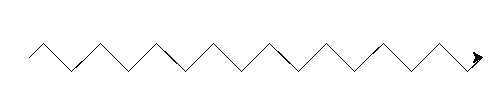
\includegraphics[width=0.5\textwidth]{img/pattern.png}
    \caption{Rectangle pattern.}
    \label{fig:enter-label}
\end{figure}

Next, experiment a bit and implement your own ideas. Following is another example of a pattern created from circles. Be creative!

\begin{figure}[!h]
    \centering
    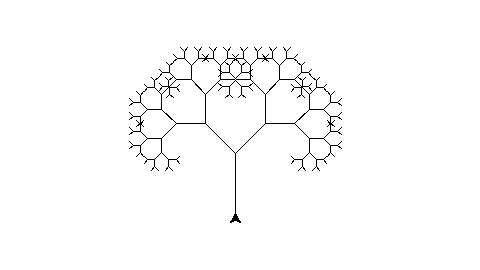
\includegraphics[width=0.5\textwidth]{img/pattern2.png}
    \caption{Circle pattern.}
    \label{fig:enter-label}
\end{figure}

\end{task}

\clearpage


\begin{task}{Recursive spiral}{}{}

Implement a recursive function \code{spiral(int: size, float: angle, float: scale, int: maxSize)} that draws spirals like the example below.

\begin{figure}[!h]
    \centering
    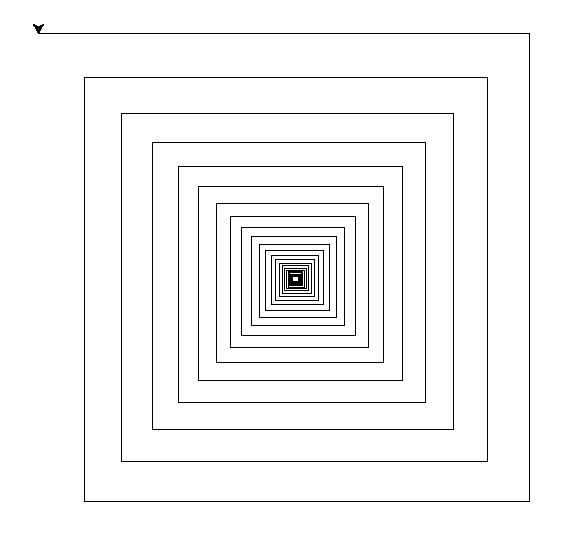
\includegraphics[width=1\textwidth]{img/spiral.png}
    \caption{A spiral.}
    \label{fig:enter-label}
\end{figure}

\end{task}

\clearpage

\begin{task}{Recursive tree}{}{}

Implement a recursive function \code{tree(int: branches, int: size, float: angle, float: scale)} that draws trees like the examples below. 

\begin{figure}[!h]
    \centering
    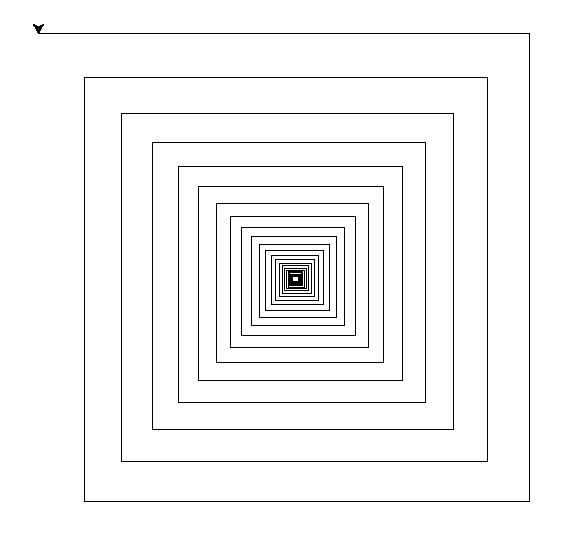
\includegraphics[width=1\textwidth]{img/tree45.png}
    \caption{A tree created with $45^{\circ}$ angles.}
    \label{fig:enter-label}
\end{figure}

\begin{figure}[!h]
    \centering
    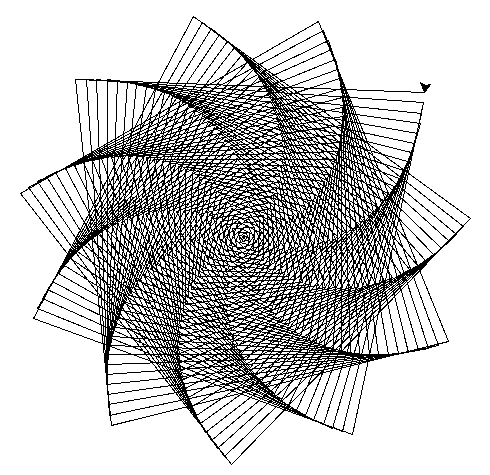
\includegraphics[width=1\textwidth]{img/tree90.png}
    \caption{A tree created with $90^{\circ}$ angles.}
    \label{fig:enter-label}
\end{figure}

\end{task}

\end{document}